\section{Ejercicio 1}
El dominio consistirá en la definición de diferentes tipos de animales junto con sus alimentos y habitats. De los animales se conocerá su nombre, tamaño promedio y peso promedio. De los alimentos se conoce su nombre y descripción. Del habitat en donde viven los animales se sabe el nombre, ubicación y clima. Los animales siempre serán o  terrestres o acuáticos, sin poder ser ambos a la vez. Ademas de los animales terrestres se pueden clasificar como cuadrúpedos o bípedos, mientras que los acuáticos se clasifican en cetáceos y peces. Finalmente de los animales acuáticos se conoce el tipo de agua en la que habitan, es decir dulce o salda
\begin{figure}[!h]
  \centering
  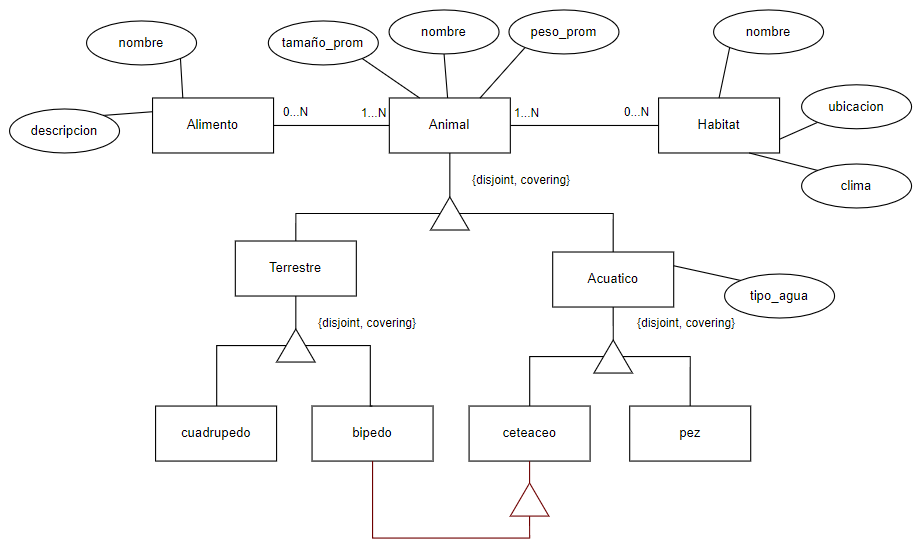
\includegraphics[width=16cm, scale=1]{Images/Imagenes/MER.png}
  \caption{Modelo entidad relación del dominio planteado junto con la inconsistencia}
  \label{fig:mer}
\end{figure}

En el MER planteado se puede observar en rojo una generalización especialización entre ``Cetaceo'' y ``Bipedo'', esta constituye una inconsistencia en el modelo debido a que las generalizaciones/especializaciones son totales y disjuntas por lo que si un ``Animal'' es ``Terrestre'' nunca podrá ser ``Acuático'' y al no poder ser ``Acuático'' entonces un ``Bipedo'' nunca debería poder ser un ``Cetaceo''. Esta relación se representa a traves de la lógica de la siguiente manera:
\begin{tcolorbox}
  Sea x un animal:
  
  \begin{center}
    $Cuadrupedo(x) \lor Bipedo(x) \longrightarrow Terrestre(x)$

    $Terreste(x) \longrightarrow \lnot Acuatico(x) $

    $Cuadrupedo(x) \longrightarrow \lnot Bipedo(x)$

    $Bipedo(x) \longrightarrow \lnot Cuadrupedo(x)$
    
    $Cetaceo(x) \lor Pez(x)\longrightarrow Acuatico(x)$

    $Acuatico(x) \longrightarrow \lnot Terrestre(x) $

    $Cetaceo(x) \longrightarrow \lnot Pez(x)$

    $Pez(x) \longrightarrow \lnot Cetaceo(x)$

    %$Terrestre(x) \land Cuadrupedo(x) \longrightarrow \lnot Bipedo(x) $
    %$Terrestre(x) \land Bipedo(x) \longrightarrow \lnot Cuadrupedo(x) $
  \end{center}
\end{tcolorbox}

Como se tiene que los ``Bipedos'' son animales ``Terrestres'' entonces se tiene que estos no pueden ser animales ``Acuaticos'' y por extension no pueden ser un ``cetaceos'', ya que si lo fueran también serian ``Acuaticos''. Por lo tanto queda claro que la especializacion/generalizacion entre ``Cetaceo'' y ``Bipedo'' no es posible dada la disyunción existente entre ``Terrestres'' y ``Acuaticos''. Por lo tanto, lo representado en rojo de la figura \ref{fig:mer} es efectivamente una inconsistencia en el modelo

\begin{tcolorbox}[title=Definicion con Lógicas Descriptivas]
\textbf{Habitat:}\\
$\exists clima \sqsubseteq Habitat$

$\exists nombre \sqsubseteq Habitat$

$\exists ubicacion \sqsubseteq Habitat$\\

\textbf{Alimento:}\\
$\exists nombre \sqsubseteq Alimento$

$\exists descripcion \sqsubseteq Alimento$\\

\textbf{Animal:}\\
$\exists nombre \sqsubseteq Animal$

$\exists peso\_prom \sqsubseteq Animal$

$\exists tamanio\_prom \sqsubseteq Animal$\\

\textbf{Terrestre:}\\
$Terrestre \sqsubseteq Animal \sqcap \lnot Acuatico$\\

\textbf{Acuatico:}\\
$Acuatico \sqsubseteq Animal \sqcap \lnot Terrestre$

$\exists tipo\_agua \sqsubseteq Acuatico$\\

\textbf{Cuadrupedo:}\\
$Cuadrupedo \sqsubseteq Terrestre \sqcap \lnot Bipedo$\\

\textbf{Bipedo:}\\
$Bipedo \sqsubseteq Terrestre \sqcap \lnot Cuadrupedo$\\

\textbf{Cetaceo:}\\
$Cetaceo \sqsubseteq Acuatico \sqcap \lnot Pez$\\

\textbf{Pez:}\\
$Pez \sqsubseteq Acuatico \sqcap \lnot Cetaceo$\\

\textbf{Relacion $\mathbf{Animal \leftrightarrow Habitat}$:}\\
$Animal \sqsubseteq \geq0 habita.Habitat$

$Habitat\sqsubseteq \exists esHabitado.Animal$\\

\textbf{Relacion $\mathbf{Animal \leftrightarrow Alimento}$:}\\
$Animal \sqsubseteq \geq0 come.Alimento$

$Alimento\sqsubseteq \exists esComido.Animal$
\end{tcolorbox}

\subsection{Validación con Protégé}
Al modelar la ontología en Protégé y validarla con el razonador HermiT, se puede detectar la presencia de inconsistencias. En la Figura 1, se muestra un ejemplo en el cual el razonador HermiT identifica una inconsistencia y proporciona una explicación para la misma.

La explicación del razonador indica que la clase ``Bipedo'' es una subclase de ``Cetaceo'', y a su vez, ``Cetaceo'' es una subclase de ``Acuatico''. Sin embargo, también se establece que ``Bipedo'' es una subclase de ``Terrestre'' y que ``Acuatico'' y ``Terrestre'' son clases disjuntas, lo que implica que no pueden tener instancias en común.

Esta explicación muestra que la existencia de ``Bipedo'' como subclase tanto de ``Cetaceo'' (que está relacionado con ``Acuatico'') como de ``Terrestre'' es contradictoria debido a la disyunción planteada entre ``Acuatico'' y ``Terrestre''. Por lo tanto, se demuestra la inconsistencia en el modelo ontológico y coincide con lo planteado a traves de la lógica previamente.

\begin{figure}[!h]
  \centering
  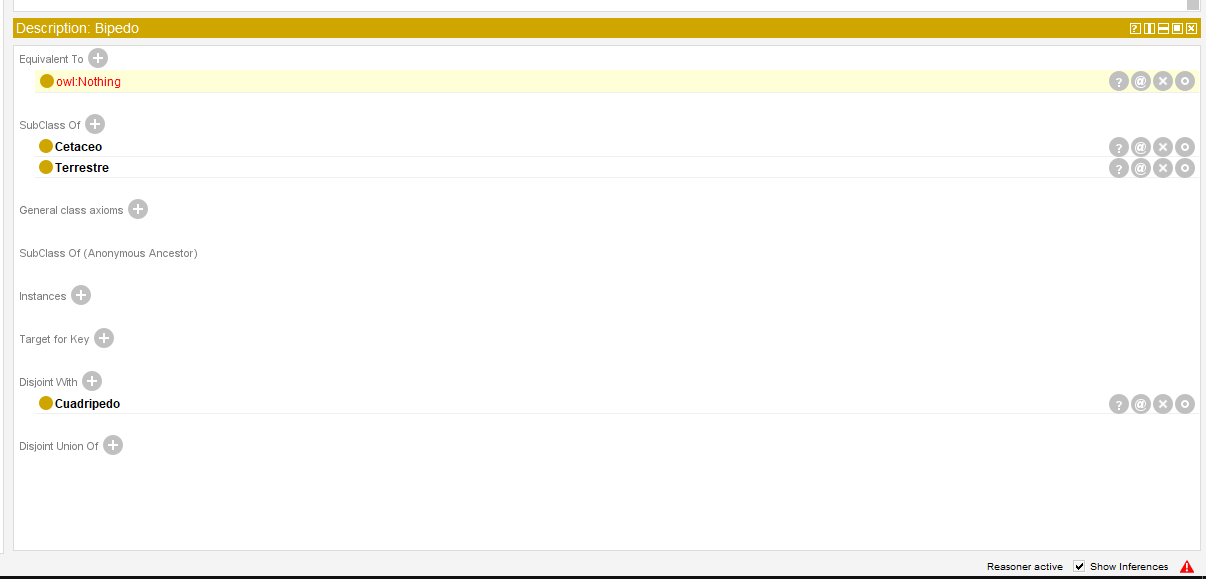
\includegraphics[width=16cm, scale=1]{Images/Imagenes/Protege1.png}
  \caption{Detección de inconsistencia en Bípedo}
  \label{fig:prot1}
\end{figure}

\begin{figure}[!h]
  \centering
  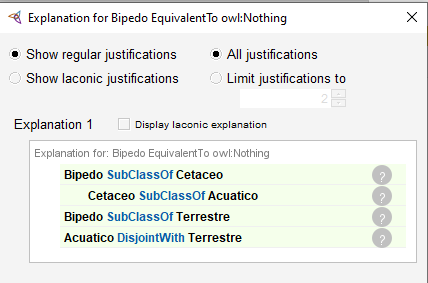
\includegraphics[width=10cm, scale=1]{Images/Imagenes/Protege2.png}
  \caption{Explicación del razonador HermiT a la inconsistencia encontrada en Bipedo}
  \label{fig:prot2}
\end{figure}

\subsection{Definición de relación en OWL y RDF}
Ademas de las diferencias sintácticas que se pueden apreciar entre las definiciones de Owl y RDF de los cuadros de mas abajo, aunque en el ejemplo planteado no se puede observar claramente, se debe destacar que OWL se basa en lógica descriptiva y permite expresar relaciones complejas y razonar sobre ellas. Ademas proporciona constructores específicos para definir jerarquías de clases, propiedades y restricciones que facilitan el razonamiento lógico.

En cambio RDF es un modelo de datos básico que se utiliza para la representación de la información
en la web semántica y no proporciona la capacidad de definir restricciones complejas o realizar razonamiento lógico directamente. RDF posee una expresividad mas limitada que OWL y se centra principalmente en la representación de tripletas sujetos-predicados-objetos sin proporcionar construcciones especificas para definir jerarquías o restricciones complejas
\begin{tcolorbox}[title=Definición en RDF de ``Acuatico'' subclase de ``Animal'' y disjunto con ``Terrestre'']
\begin{lstlisting}[language=XML, breaklines=true]
  <owl:Class rdf:about="http://tpo1#Animal">
      <rdfs:subClassOf rdf:resource="http://www.w3.org/2000/01/rdf-schema#Class"/>
  </owl:Class>
  
  <owl:Class rdf:about="http://tpo1#Acuatico">
      <rdfs:subClassOf rdf:resource="http://tpo1#Animal"/>
      <owl:disjointWith rdf:resource="http://tpo1#Terrestre"/>
  </owl:Class>
  
  <owl:Class rdf:about="http://tpo1#Terrestre">
      <rdfs:subClassOf rdf:resource="http://www.w3.org/2000/01/rdf-schema#Class"/>
  </owl:Class>
\end{lstlisting}
\end{tcolorbox}

\begin{tcolorbox}[title=Definición en RDF de ``Acuatico'' subclase de ``Animal'' y disjunto con ``Terrestre'']
  \begin{lstlisting}[language=XML, breaklines=true]
  <rdf:Description rdf:about="http://tpo1#Animal">
    <rdf:type rdf:resource="http://www.w3.org/2000/01/rdf-schema#Class"/>
  </rdf:Description>

  <rdf:Description rdf:about="http://tpo1#Acuatico">
    <rdf:type rdf:resource="http://www.w3.org/2000/01/rdf-schema#Class"/>
    <rdfs:subClassOf rdf:resource="http://tpo1#Animal"/>
    <rdfs:disjointWith rdf:resource="http://tpo1#Terrestre"/>
  </rdf:Description>

  <rdf:Description rdf:about="http://tpo1#Terrestre">
    <rdf:type rdf:resource="http://www.w3.org/2000/01/rdf-schema#Class"/>
  </rdf:Description>

  \end{lstlisting}
  \end{tcolorbox}

